\documentclass{beamer}
\usepackage{verbatim}
\usepackage{amsmath}
\usepackage{euler}
\usepackage{graphicx}
\usepackage{subcaption}
\usepackage{hyperref}
\usetheme[progressbar = frametitle]{metropolis}
\setbeamertemplate{frame numbering}[fraction]
\title{Decoherence Corrections in TSH}
\author{Elious}
\date{}

\begin{document}
\metroset{block=fill}
	\begin{frame}
	\titlepage
	\end{frame}
	\begin{frame}[t]{Lets recap the Double slit experiment}
	\begin{center}
	\begin{figure}
	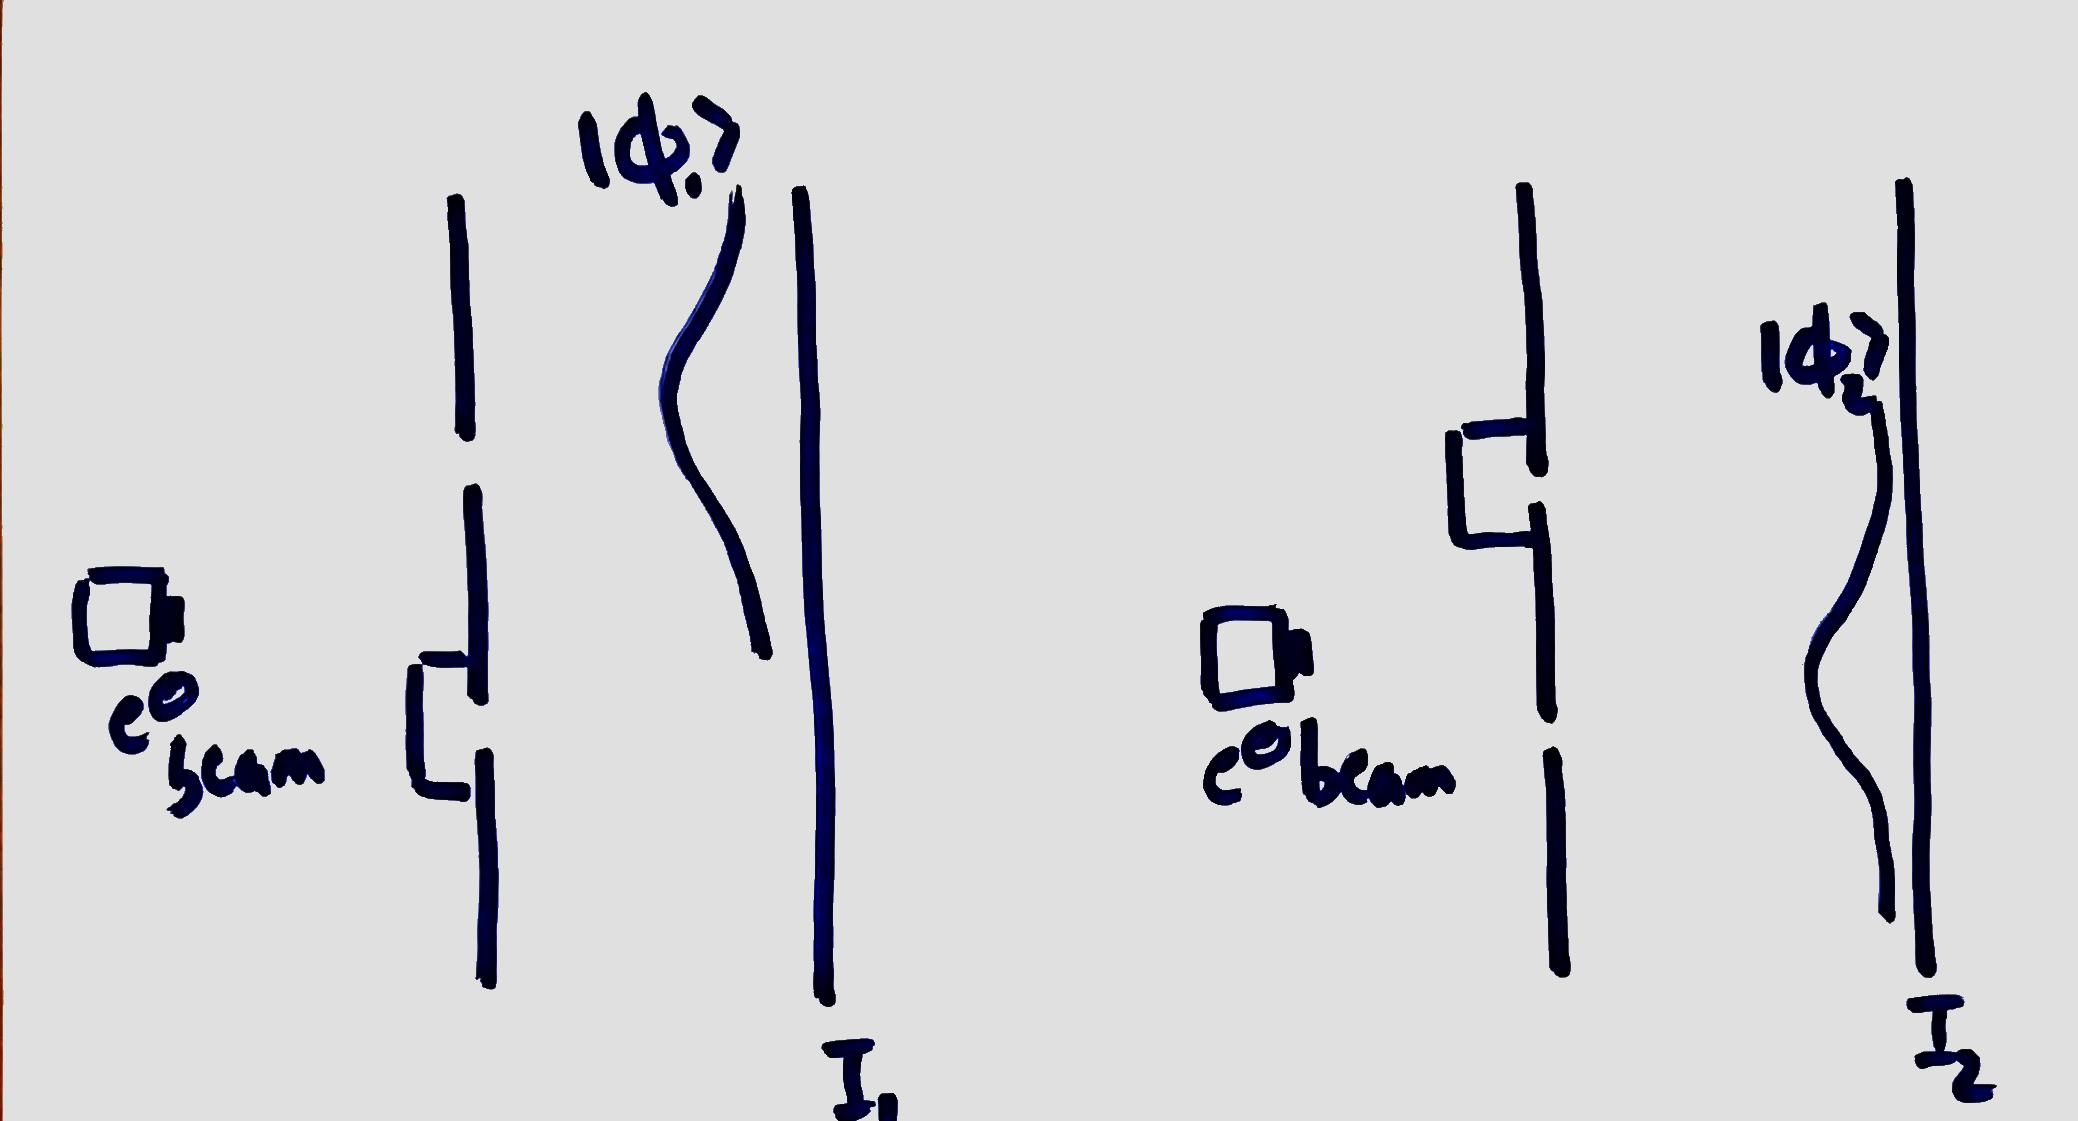
\includegraphics[scale=0.15]{initial_cases.jpg}
	\caption{One of the slits is open}
	\end{figure}
	\end{center}
	\end{frame}
	
	\begin{frame}[t]{Double slit experiment results}
	\begin{center}
	\begin{figure}
	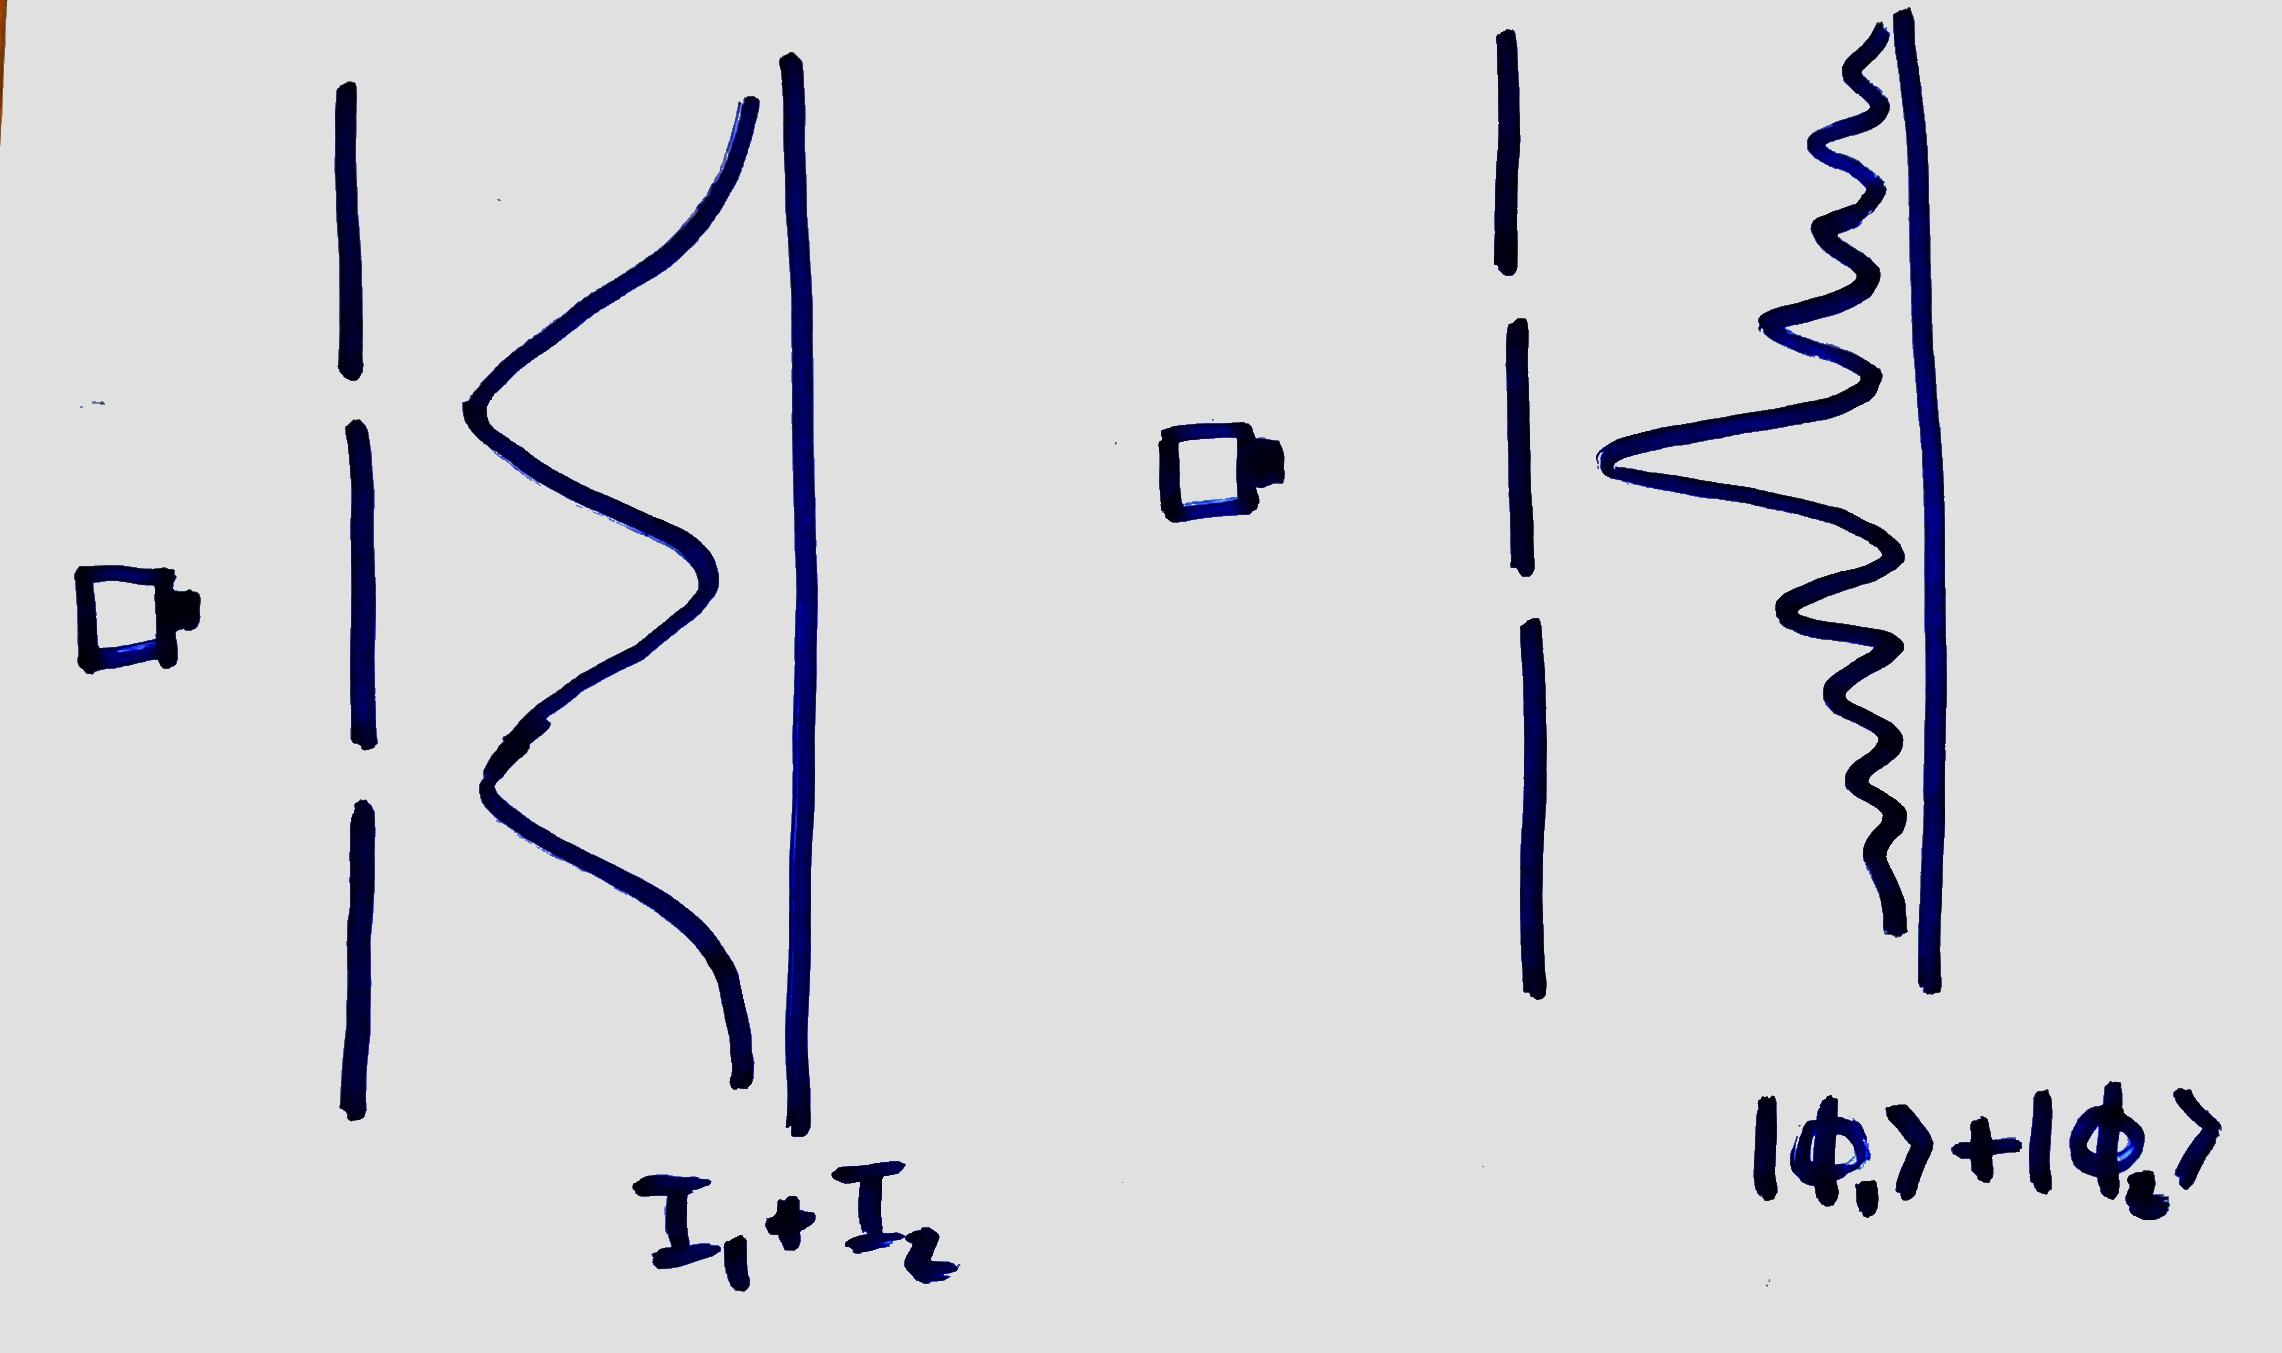
\includegraphics[scale=0.12]{classical_vs_quantum.jpg}
	\caption{Both slits open: left $\rightarrow$ Classical expectation, right $\rightarrow$ Quantum reality}
	\end{figure}
	\end{center}
	\end{frame}
	
	\begin{frame}[t]{So what is going on?}
	\begin{flushleft}
	\begin{large}
	Instead of the intensities, the quantum amplitude gets added up and we have :
	\begin{equation}\label{eq:1}
	|\Psi\rangle = c_1|\phi_1\rangle + c_2|\phi_2\rangle
	\end{equation}
	and the intensity is given by:
	\begin{equation}\label{eq:2}
	\begin{split}
	\langle\Psi|\Psi\rangle &= |c_1|^2\langle\Phi_1|\Phi_1\rangle + |c_2|^2\langle\Phi_2|\Phi_2\rangle +\\ & \ \ \ \ c_1^*c_2\langle\Phi_1|\Phi_2\rangle + c_1c_2^*\langle\Phi_2|\Phi_1\rangle
	\end{split}
	\end{equation}
	The last two terms are what gives rise to the interference and sometimes also called \textbf{coherence} 
	\end{large}
	\end{flushleft}
	\end{frame}		
	
	\begin{frame}[t]{Lets take quick look at the expansion of infinite well}
	\begin{figure}
	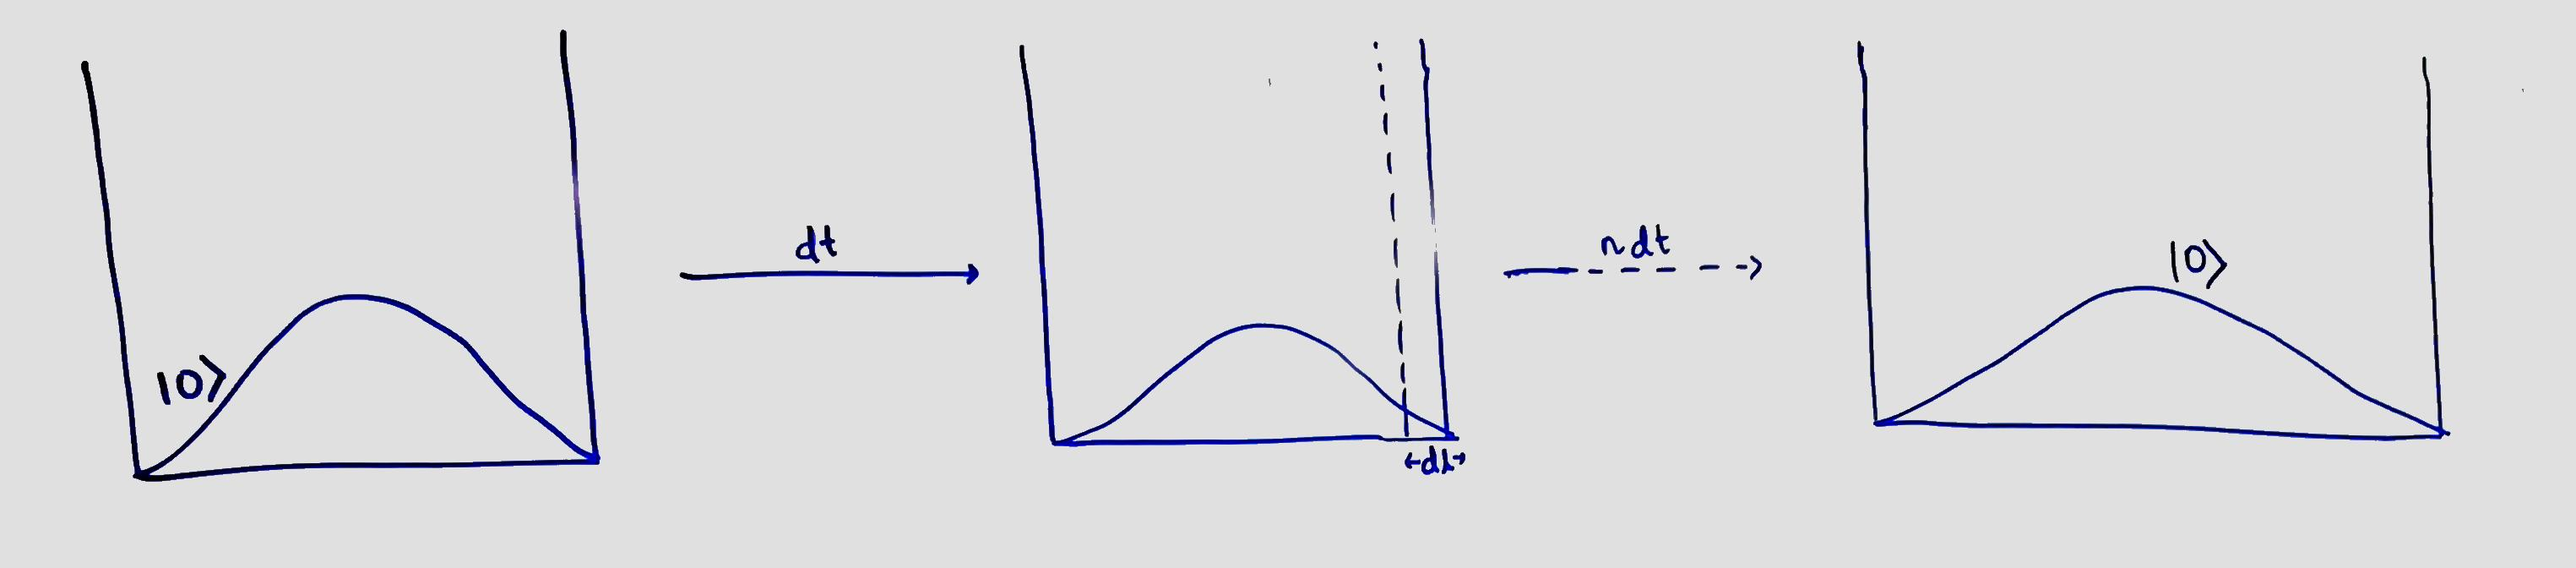
\includegraphics[scale=0.1]{adiabatic_infinite_well.jpg}
	\caption{Slow (Adiabatic) expansion of the well}
	\end{figure}
	\begin{figure}
	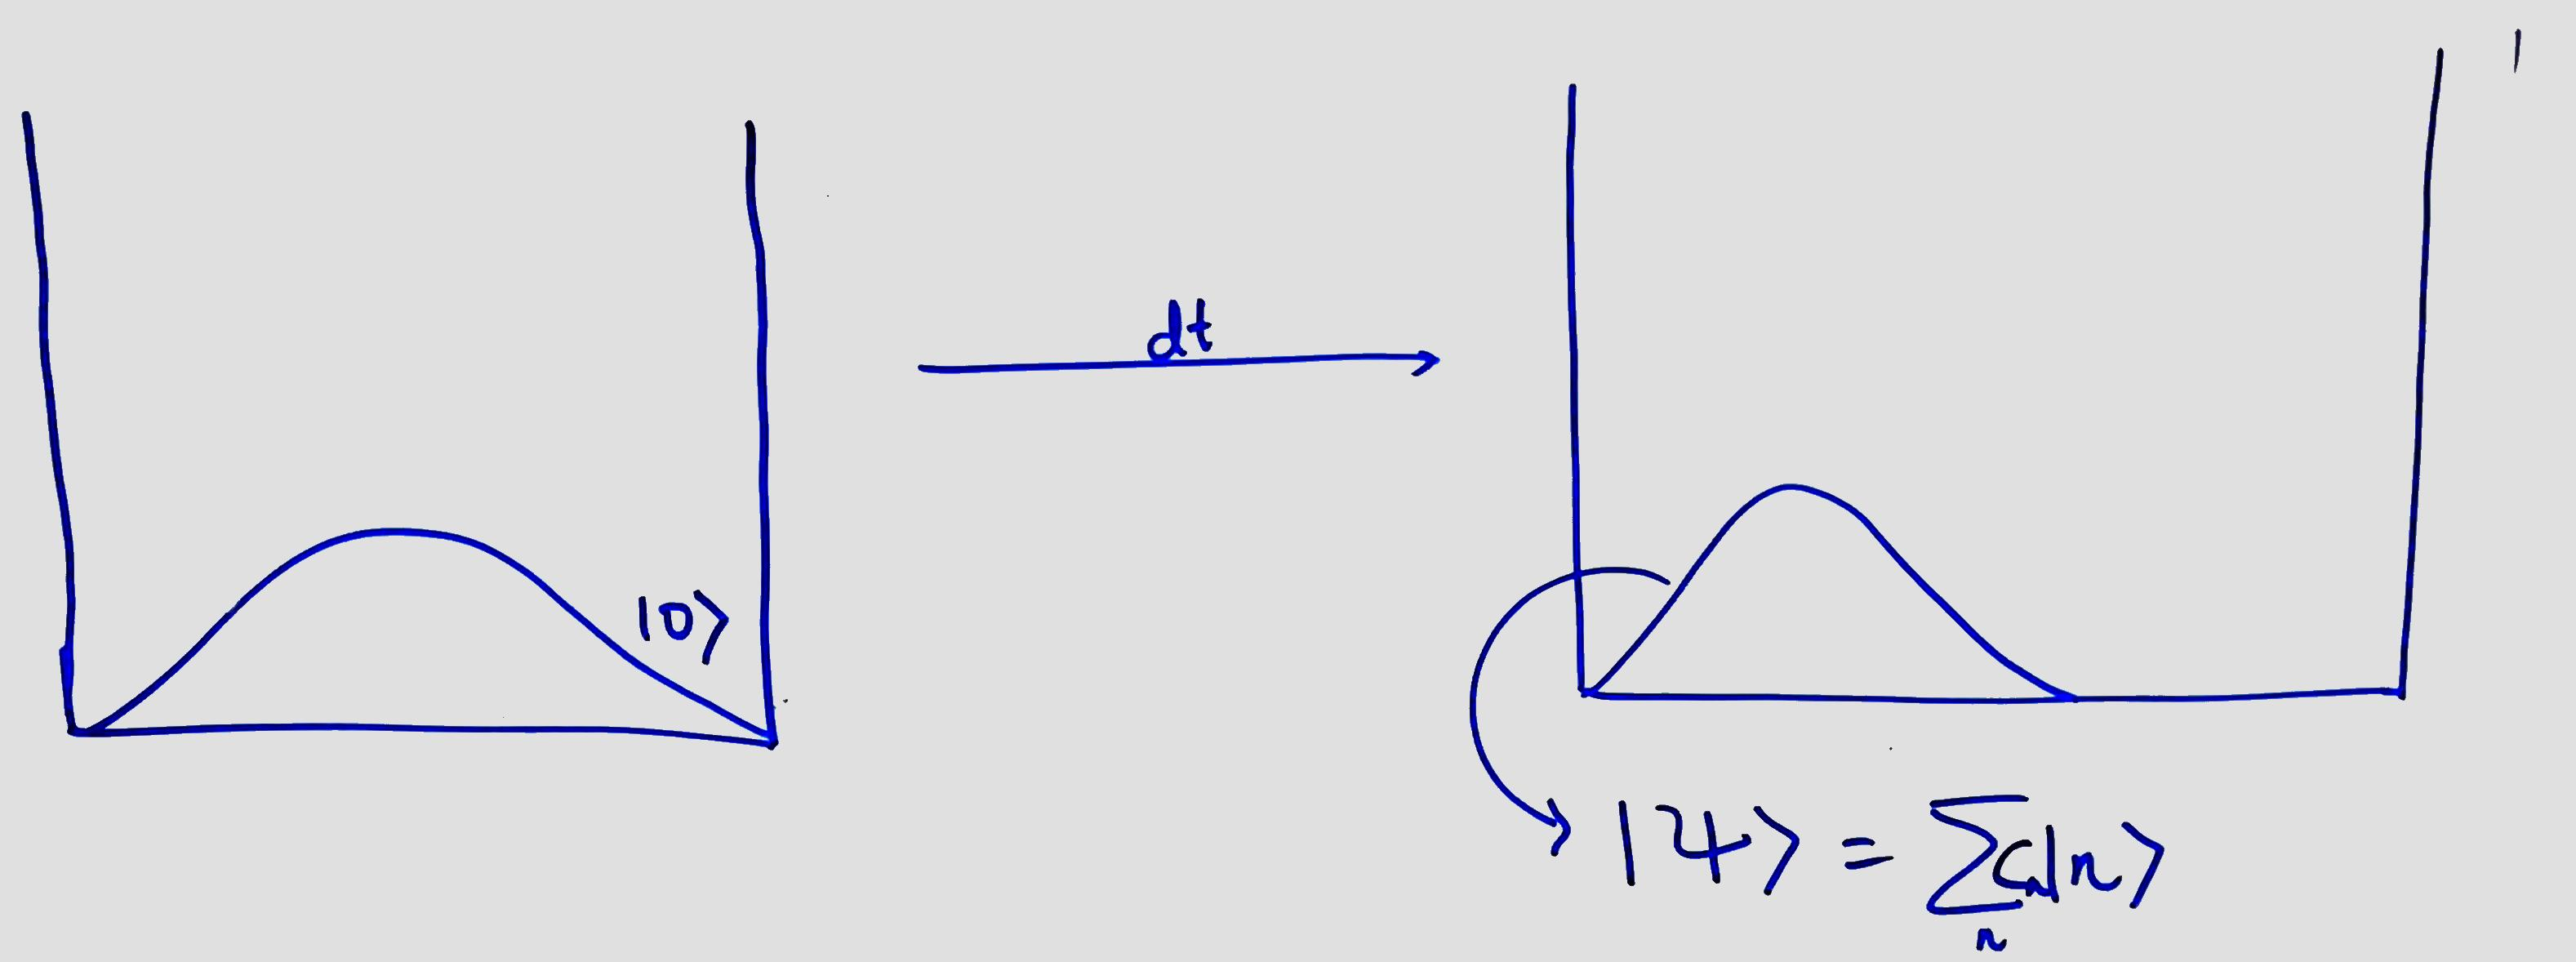
\includegraphics[scale=0.065]{nonadiabatic_infinite_well.jpg}
	\caption{Sudden (Non-adiabatic) expansion of the well}
	\end{figure}
	\end{frame}
	
	\begin{frame}[t]{Coherence}
	Sudden expansion $\rightarrow$ System can't adapt and the resulting wavefunction is now : 
	\begin{equation}\label{eq:3}
	|\Psi\rangle = \sum_nc_n|\phi_n\rangle
	\end{equation}
	If we construct the density matrix:
	\begin{equation}\label{eq:4}
	|\Psi\rangle\langle\Psi| = \begin{pmatrix}
c_1c_1^* & c_1c_2^* & ... & c_1c_n^*\\
c_2c_1^* & c_2c_2^* & ... & c_2c_n^*\\
\vdots & \vdots & \ddots & \vdots \\
c_nc_1^* & c_nc_2^* & ... & c_nc_n^*\\
\end{pmatrix}
	\end{equation}
	Diagonal terms $\rightarrow$ \textbf{Populations}\\
	Off-diagonal terms $\rightarrow$ \textbf{Coherence} $\rightarrow$ reason for interference patterns and a measure of how much one state interferes with the other states.
	\end{frame}		
	
	\begin{frame}[t]{Just a recap of TSH}
	The basic priciple is that the nuclear coordinates and traverse classically along an adiabatic surface by:
	\begin{equation}\label{eq:5}
	M_I\ddot{\textbf{R}} = -\nabla E_k^{el}(\textbf{R})
    \end{equation}
    and the electronic coefficients are propagated according to 
    \begin{equation}\label{eq:6}
    i\hbar\dot{c}_k^\alpha(t) = c_k^\alpha(t)E_k^\alpha(\textbf{R}^\alpha) - i\hbar \sum_jc_j^\alpha \textbf{d}_{kj}^\alpha \textbf{.}\dot{\textbf{R}^\alpha}
    \end{equation}
    The hops are allowed between different PES only when:
    \begin{equation}\label{eq:7}
    \sum_{m=1}^{k-1}P_{j\rightarrow m} < \zeta <  \sum_{m=1}^{k}P_{j\rightarrow m}
    \end{equation}    
    where $P_{j\rightarrow m}$ just depends on the Non-adiabatic coupling in eqn(\ref{eq:6}) and $\zeta$ is a random number within $(0,1)$.	 
	\end{frame}
	
	\begin{frame}[t]{Over-coherence in TSH}
	\begin{center}
	\begin{figure}
	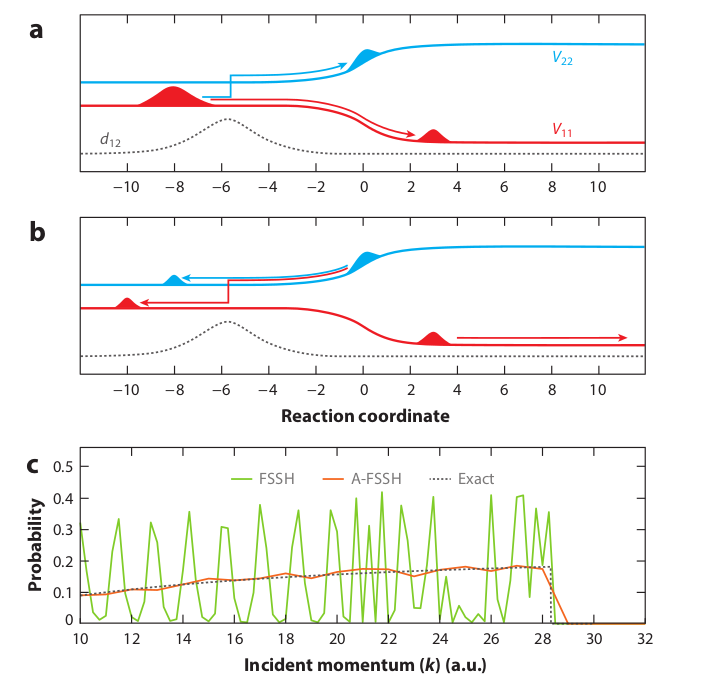
\includegraphics[scale=0.40]{tully_model_3.png}
	\caption{(c) Probability of reflection to lower
surfaces}
	\end{figure}
	\end{center}
	\end{frame}
	
	\begin{frame}[t]{Why overcoherence happens???}
	Consider the Born-Huang ansatz for total wavefunction of the combined nuclei-electron system:
	\begin{equation}\label{eq:8}
	|\Psi\rangle = \sum_i |\chi_i\rangle|\phi_i\rangle 
	\end{equation}
	The density matrix will be;
	\begin{equation}\label{eq:9}
	|\Psi\rangle\langle\Psi| = \sum_{i,j} |\chi_i\rangle|\phi_i\rangle \langle\phi_j|\langle\chi_j|
	\end{equation}
	Now to bring out the electronic density matrix from this;
	\begin{equation}\label{eq:10}
	\sigma_{el} = \sum_{i,j} \displaystyle\int|\textbf{R}\rangle\langle\textbf{R}||\Psi\rangle\langle\Psi| d\textbf{R}
	\end{equation}
	\end{frame}

	\begin{frame}[t]{Overcoherence...}
	This would give;
	\begin{equation}\label{eq:11}
	\begin{split}
	\sigma_{el} &= \sum_{i,j} \displaystyle\int \langle\chi_j|\textbf{R}\rangle\langle\textbf{R}|\chi_i\rangle|\phi_i\rangle\langle\phi_j| d\textbf{R}\\
	&= \sum_{i,j} \langle\chi_j|\chi_i\rangle|\phi_i\rangle\langle\phi_j|
	\end{split}
	\end{equation}
	The electronic wavefunction in TSH is;
	\begin{equation}\label{eq:12}
	|\Psi_{el}\rangle = \sum_i c_i|\phi_i\rangle
	\end{equation}
	From this we have the electronic density matrix as;
	\begin{equation}\label{eq:13}
	\sigma_{el} = \sum_{i,j} c_ic_j^*|\phi_i\rangle\langle\phi_j|
	\end{equation}
    \end{frame}	
    
    \begin{frame}[t]{Overcoherence continued...}
    Comparing equations (\ref{eq:11}) and (\ref{eq:13}) we can see that the coherence terms in TSH wave-function  represents the nuclear overlap of the total-wavefunction, i.e.,
    \begin{equation}\label{eq:14}
    \langle\chi_j|\chi_i\rangle = c_ic_j^*
    \end{equation} 
    \begin{enumerate}
    \item{After branching off of the nuclear wavepackets from strong coupling regions, when these wavepackets are far enough in phase space, then the effective overlap should go to 0 i.e., $\langle\chi_j|\chi_i\rangle \rightarrow 0$.}
    \item{BUT, there is no term in equation(\ref{eq:6}) which will make the coherence terms $\rightarrow 0$ after the hops.}
    \item{This leads to overcoherence.}
	\end{enumerate}        
    \end{frame}    	
	
	\begin{frame}[t]{What should be happening ideally...}
	\begin{enumerate}
	\item{In strong coupling regions, the nuclear wavepackets can branch into multiple wavepackets}
	\item{Following a hop, the wavepackets remain in region of nonadiabatic coupling and continue exchanging populations.}
	\item{After enough seperation of the wavepackets in phase-space, these should evolve independent of each other.}
	\item{At ant time we should have:
	\begin{equation}\label{eq:15}
	\frac{N^\alpha}{N^T} = \frac{1}{N^T}\sum_{j=1}^{N^T} \rho_{\alpha\alpha}^j
	\end{equation}
	This is called internal consistency of FSSH.}
	\end{enumerate}
	\end{frame}
	
	\begin{comment}
	\begin{frame}[t]{What actually happens...}
	\begin{enumerate}
	\item{The equations of motion for quantum coefficients (eqn. \ref{eq:6})are propagated coherently.}
	\item{At regions of strong coupling, if the wavepacket branches into subpackets, the subpackets also begin to evolve coherently in time}
	\item{BUT they should be evolving independently, after enough seperation in phase space $\rightarrow$ \textbf{electronic decoherence}.}
	\end{enumerate}
	
	To account for decoherence some \textit{ad-hoc} methods have been developed.
	\end{frame}
	\end{comment}	
	
	\begin{frame}[t]{Instantaneous Decoherence Correction (IDC)}
	\begin{enumerate}
	\item{\textbf{ID-S:} After each successful hop, the electronic wavefunction is reinitialised as a pure state in the current state}
	\item{\textbf{ID-A:} If a hop is accepted, the wavefunction is made to collapse at the current state and if a hop is forbidden, the wavefunction is collapsed back to the current running state.}
	\end{enumerate}
	If a hop $S_2 \rightarrow S_1$ is predicted:\\
	\hspace{2cm} if successful hop:\\
	\hspace{4cm} set $c_1 = 1$ and $c_2 = 0$\\
	\hspace{2cm} else:\\
	\hspace{4cm} set $c_2 = 1$ and $c_1 = 0$\\
	\end{frame}
	
	\begin{frame}[t]{Energy Based Decoherence Correction (EDC)}
	Instead of instantaneous collapse, here we allow for decay of the electronic wavefunction to a particular state.
	\begin{equation}\label{eq:16}
	c_\beta'(t) = c_\beta(t)e^{\frac{-\Delta t}{\tau_{\beta\alpha}(t)}}
    \end{equation}
    and the loss gets accumulated in the current state as:
    \begin{equation}\label{eq:17}
    c_\alpha'(t) = c_\alpha(t)\left[\frac{1-\sum_{\beta\neq\alpha}|c_\beta'(t)|^2}{|c_\alpha'(t)|^2}\right]^{\frac{1}{2}}
    \end{equation}    	 
    $\tau_{\beta\alpha}$ is known as the decoherence time and Truhlar \textit{et al.} suggested it to be:
    \begin{equation}\label{eq:18}
    \tau_{\beta\alpha}(t) = \frac{\hbar}{|E_\beta(t)-E_\alpha(t)|}\left(C+\frac{E_0}{(\textbf{P}\textbf{.}\textbf{d}_{\alpha\beta})^2/2\mu}\right)
    \end{equation}
    Later on Granucci \textit{et al.} found, this can be approximated as:
    \begin{equation}\label{eq:19}
    \tau_{\beta\alpha}(t) = \frac{\hbar}{|E_\beta(t)-E_\alpha(t)|}\left(C+\frac{E_0}{E_{kin}}\right)
    \end{equation}
	\end{frame}
	
	\begin{frame}[t]{Visualisation of the Decoherence corrections}
	\begin{figure}
	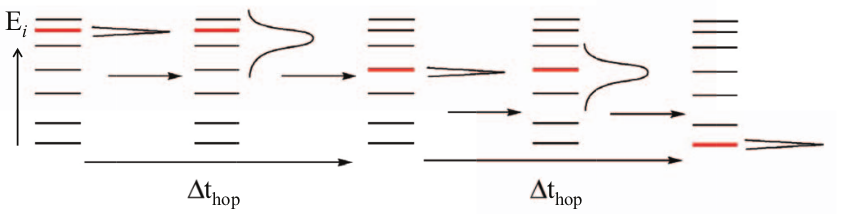
\includegraphics[scale=0.5]{IDC.png}
	\caption{Instantaneous Decoherence Correction}
	\end{figure}
	\begin{figure}
	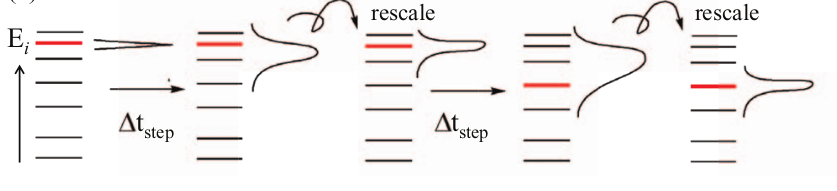
\includegraphics[scale=0.5]{EDC.png}
	\caption{Energy Based Decoherence Correction}
	\end{figure}
	\end{frame}
	
\end{document}